\appendix
\chapter{Appendix}

\section{Other Sequences}\label{sec:appendix_real_sequences}
    \begin{figure}[h]
        \centering
        \begin{subfigure}{.2\textwidth}
        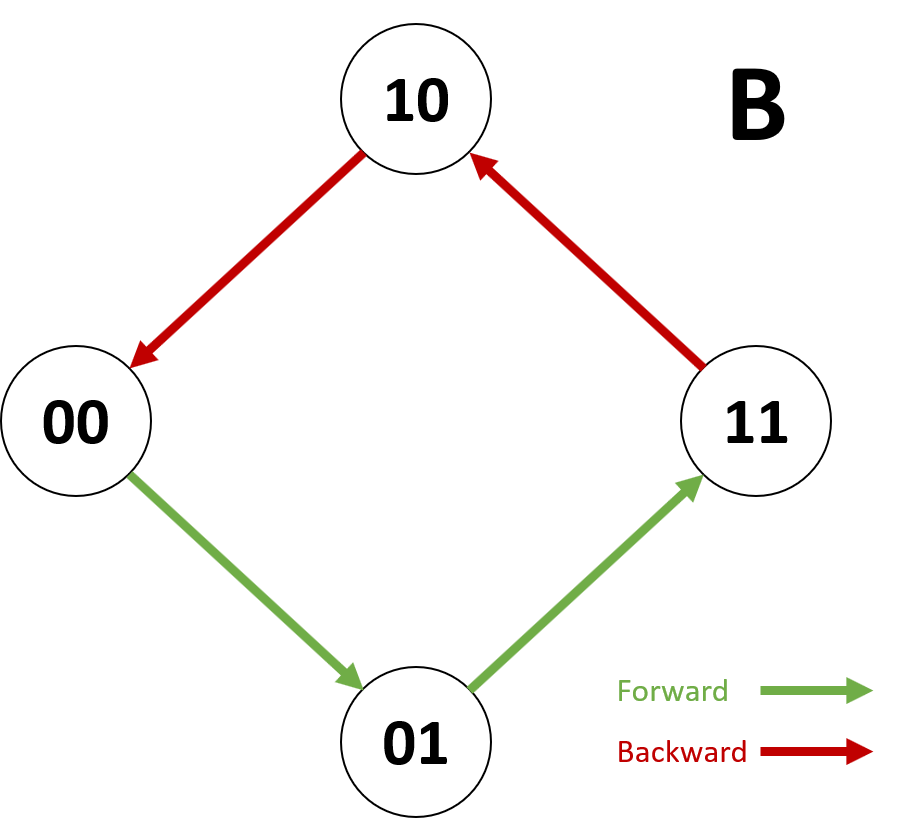
\includegraphics[width=\textwidth]{images/S_B.png}
        \end{subfigure}%
        \begin{subfigure}{.6\textwidth}
        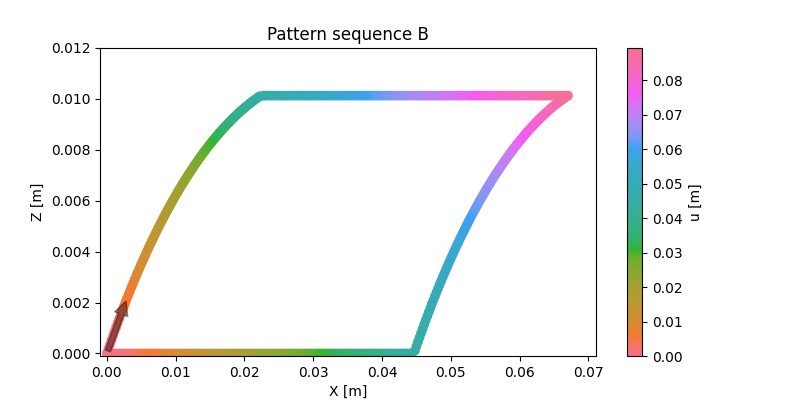
\includegraphics[width=\textwidth]{images/B.png}
        \end{subfigure}
        \caption{Sequence B is one of the simplest sequence where the top block is moving first in forward and backward motion. This leads to a hysteresis as we can see. The arrow shows the direction of motion, which is clockwise.}
        \label{fig:appendix_seq_B}
    \end{figure}
    
    \begin{figure}[h]
        \centering
        \begin{subfigure}{.2\textwidth}
        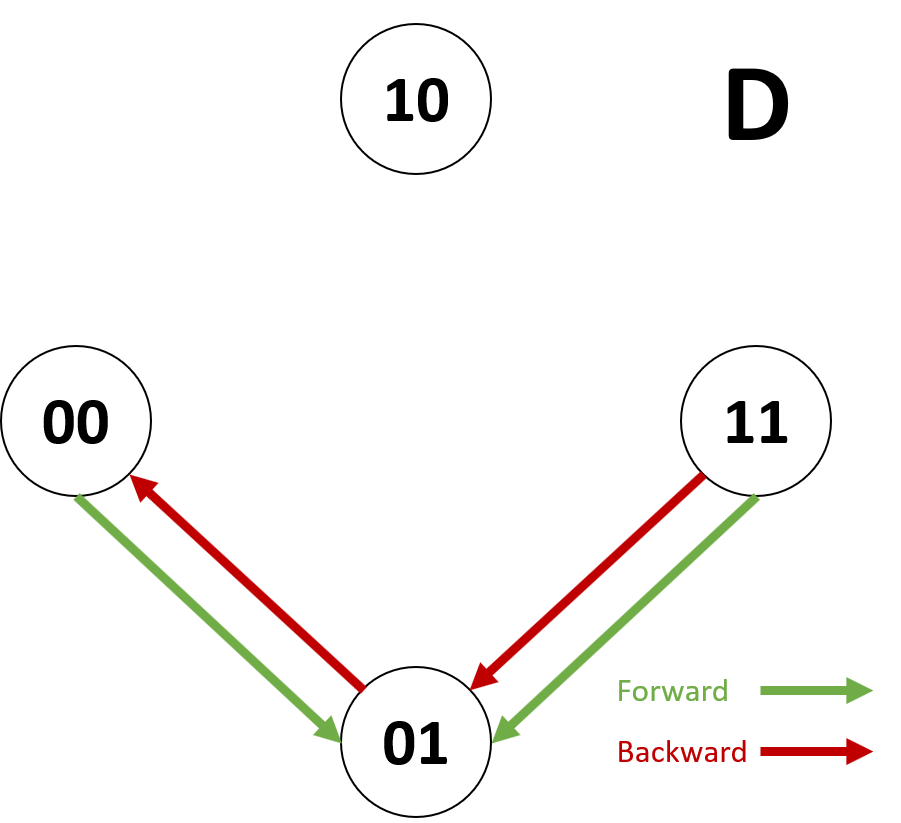
\includegraphics[width=\textwidth]{images/S_D.png}
        \end{subfigure}%
        \begin{subfigure}{.6\textwidth}
        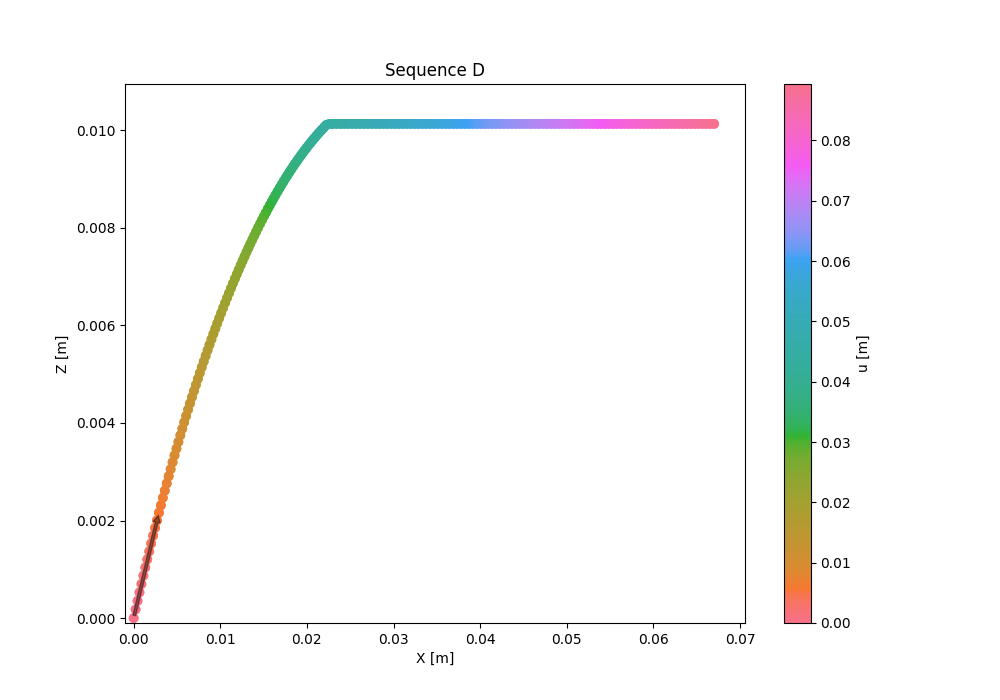
\includegraphics[width=\textwidth]{images/D.png}
        \end{subfigure}
        \caption{Sequence D is a symmetrical sequence where the forward and backward motion are following the same path. In this sequence we have first the top block moving during the forward motion where the middle block is moving first during the backward motion.}
        \label{fig:appendix_seq_D}
    \end{figure}
    
    \begin{figure}[h]
        \centering
        \begin{subfigure}{.2\textwidth}
        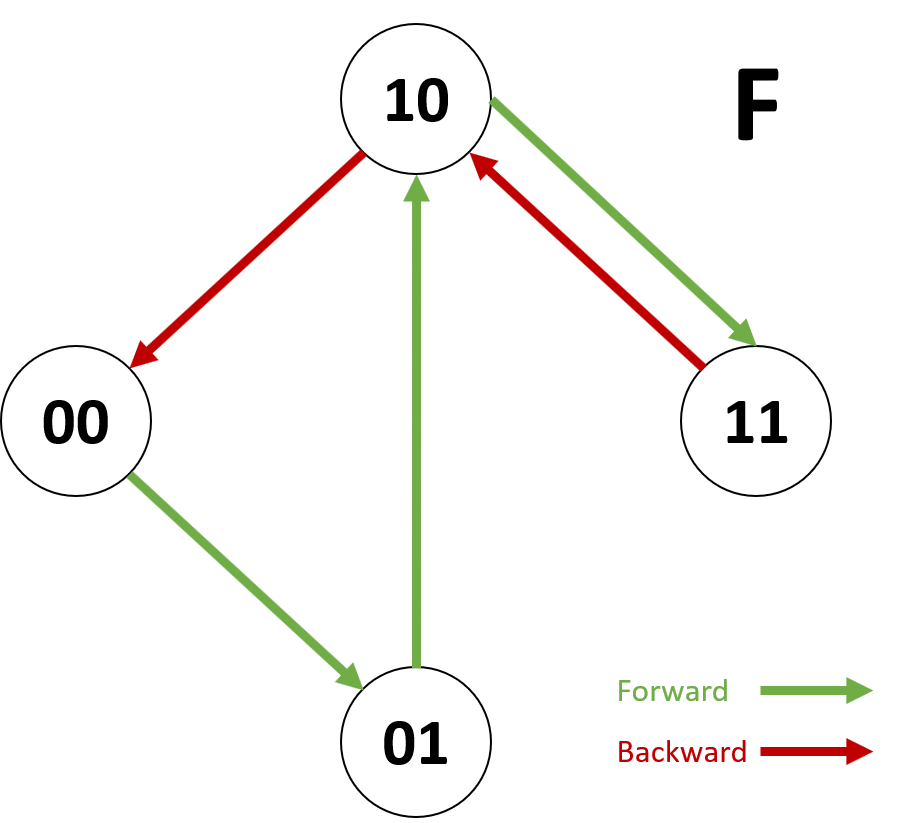
\includegraphics[width=\textwidth]{images/S_F.png}
        \end{subfigure}%
        \begin{subfigure}{.6\textwidth}
        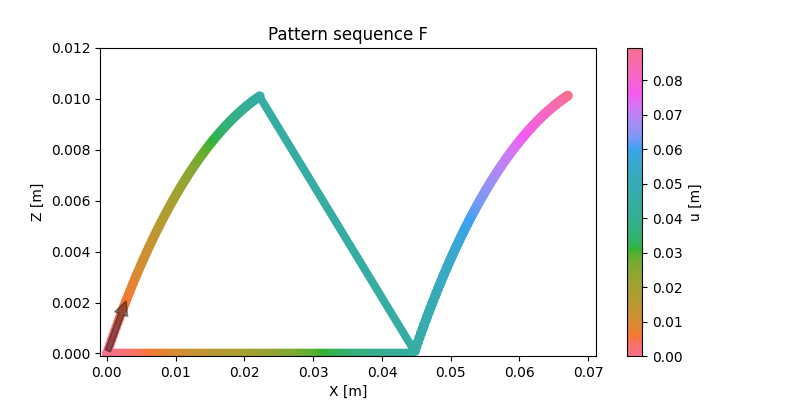
\includegraphics[width=\textwidth]{images/F.png}
        \end{subfigure}
        \caption{Sequence F is a sequence with a avalanche mechanism where two blocks swap positions. This happens in the middle of the forward motion.}
        \label{fig:appendix_seq_F}
    \end{figure}
    
    \begin{figure}[h]
        \centering
        \begin{subfigure}{.2\textwidth}
        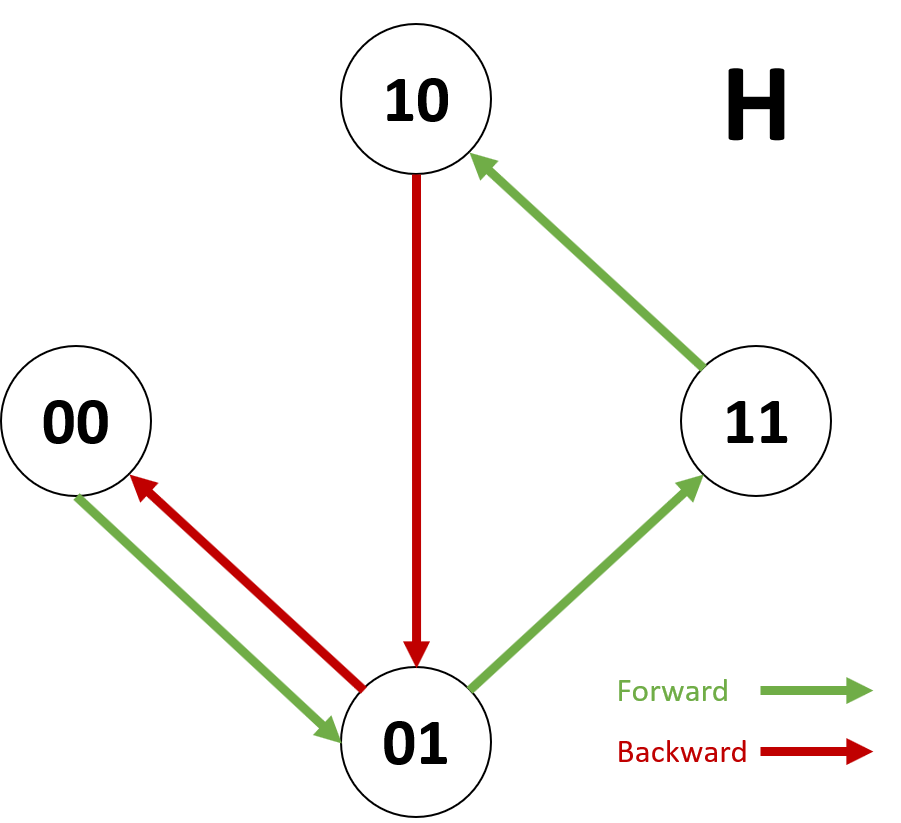
\includegraphics[width=\textwidth]{images/S_H.png}
        \end{subfigure}%
        \begin{subfigure}{.6\textwidth}
        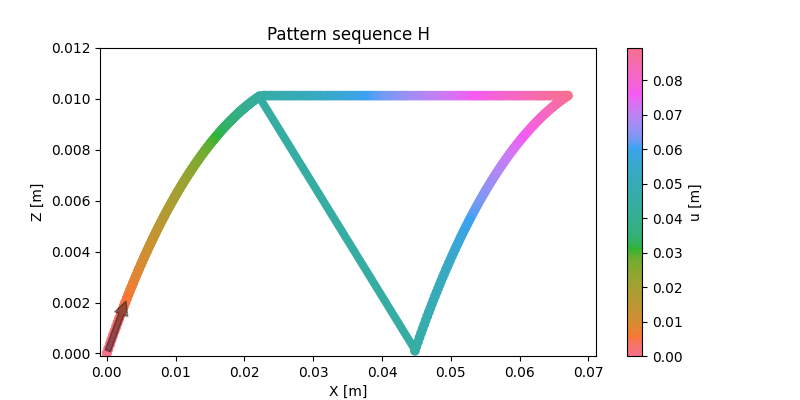
\includegraphics[width=\textwidth]{images/H.png}
        \end{subfigure}
        \caption{Sequence H is similar to sequence E and sequence F as there is also an avalanche effect that swap two blocks positions. But this time this swap motion happens during backward actuation instead of forward actuation.}
        \label{fig:appendix_seq_H}
    \end{figure}

\section{Theoretical sequences}\label{sec:appendix_sequences}
    We have different sequences that are possible in a theory but will never happens in real cases scenarios. Those cases generally implies that the two springs have exactly the same stiffness. We can see those sequences on Figure \ref{fig:sequence_impossible}. They all require two blocks to displace at the same time and in the same direction. Although they are not possible in real life, they are implemented in the simulation.
    
    \begin{figure}
    \centering
        \begin{tabular}{ccc}
            \subfloat[Sequence K]{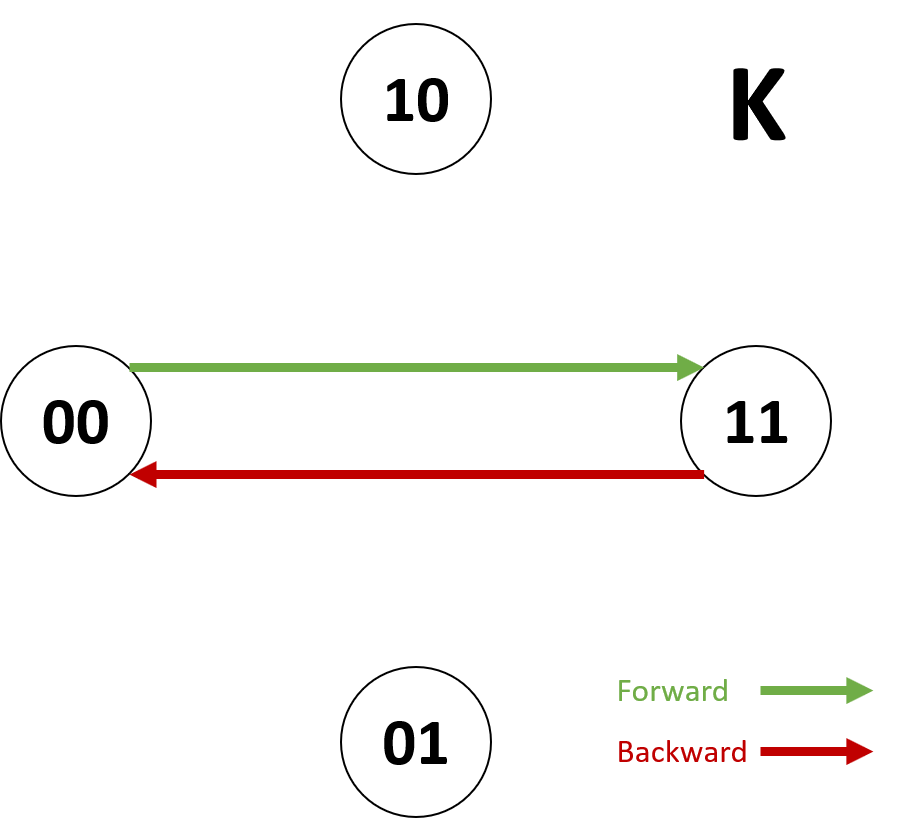
\includegraphics[width = 1.5in]{images/S_K.png}} &
            \subfloat[Sequence L]{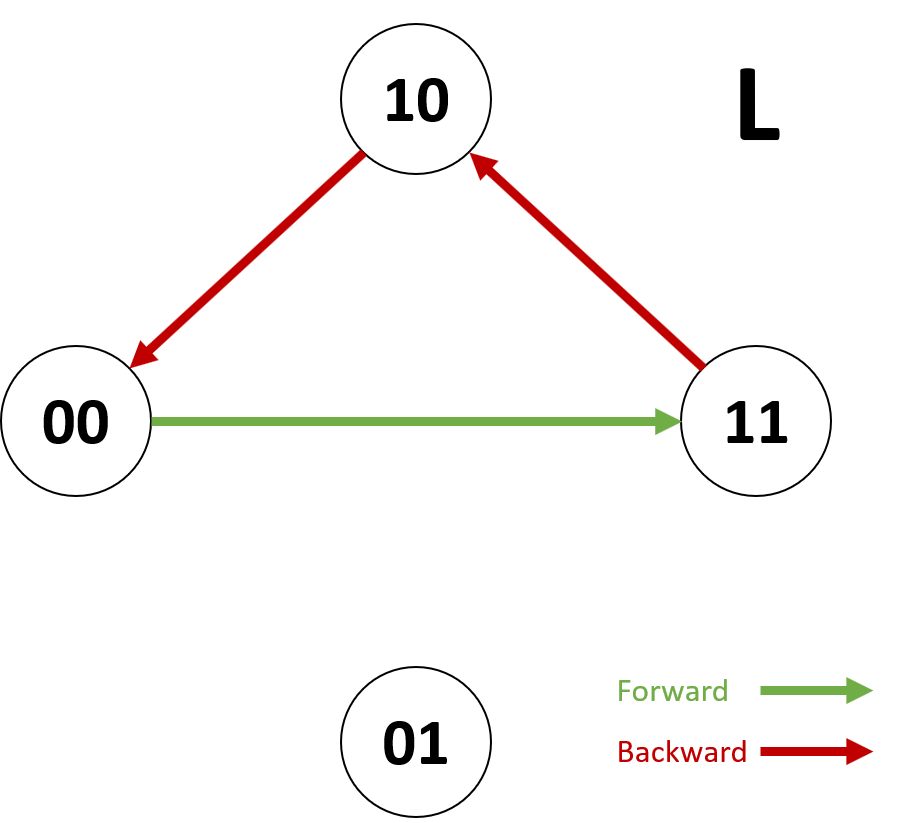
\includegraphics[width = 1.5in]{images/S_L.png}} &
            \subfloat[Sequence M]{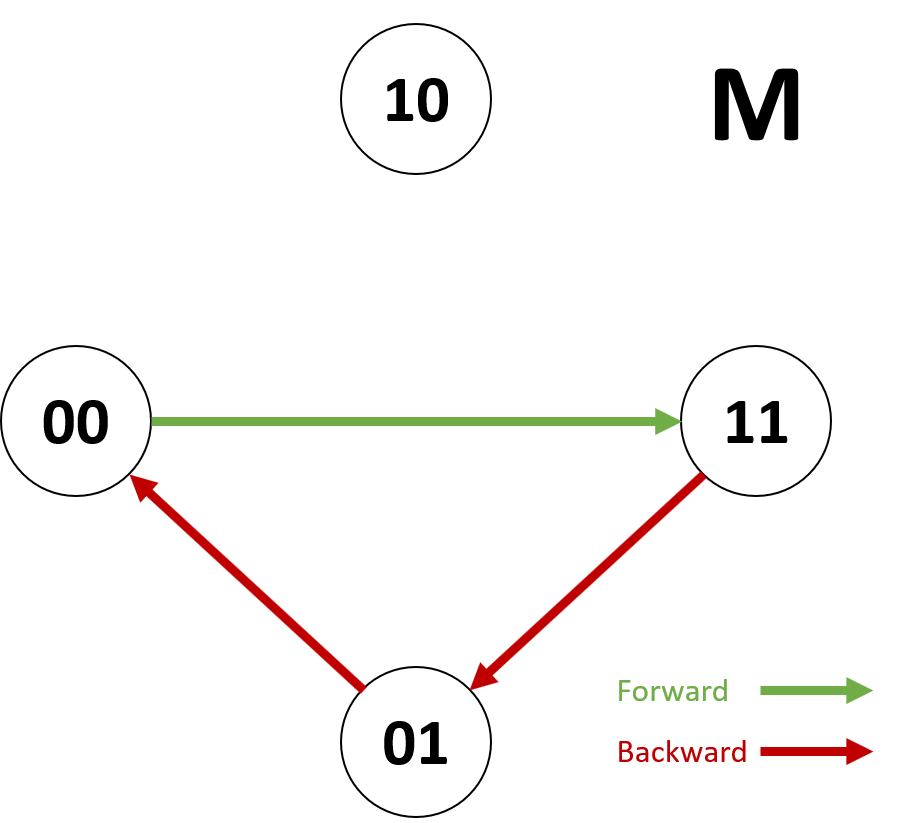
\includegraphics[width = 1.5in]{images/S_M.png}} \\
            \subfloat[Sequence N]{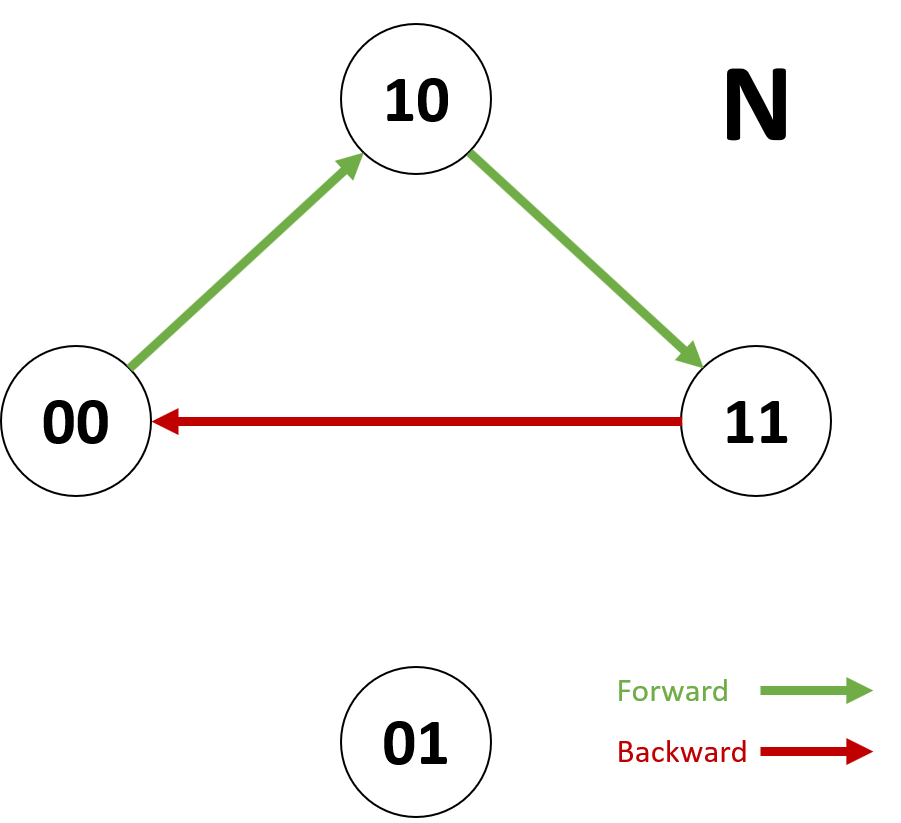
\includegraphics[width = 1.5in]{images/S_N.png}} &
            \subfloat[Sequence O]{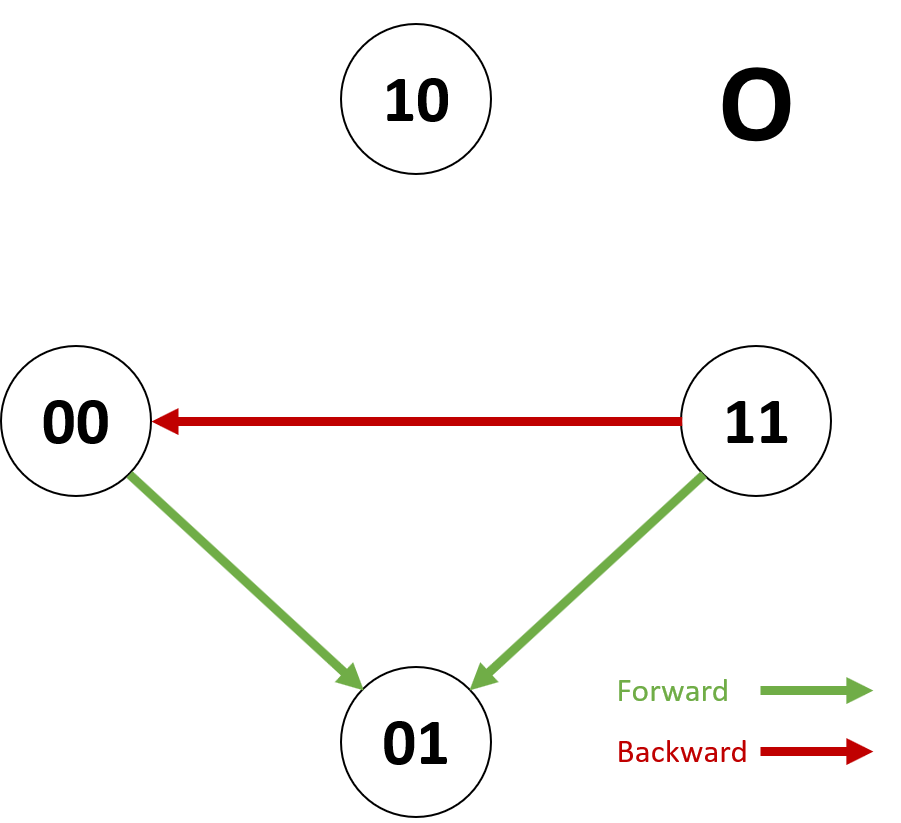
\includegraphics[width = 1.5in]{images/S_O.png}} &
        \end{tabular}
        \caption{Theoretical sequences of the multistable joint that are not possible in real life as it asks to have perfectly balanced springs and same friction in all the joints.}
        \label{fig:sequence_impossible}
    \end{figure}
    
\clearpage
\section{Configuration file}\label{sec:program_structure}
    As seen on section \ref{sec:config}, we use a JSON configuration file to load our simulation structure. An example of the JSON file is provided here:
    

% MINTED

\definecolor{keycolor}{HTML}{569CD6}
\definecolor{valuecolor}{HTML}{FFA500}

\lstdefinelanguage{js}{
  keywords={simulation, camera_robot_ref, actuation, steps, cycles, phase, draw, robot, J1, J2, J3, J4, sequence, invert_y, invert_init_angle},
  keywordstyle=\color{keycolor}\bfseries,
  keywords=[2]{true, false},
  keywordstyle=[2]\color{valuecolor}\bfseries,
  sensitive=false,
  morecomment=[s]{/*}{*/}
}

\lstset{
   language=js,
   frame=single,
   extendedchars=true,
   basicstyle=\footnotesize\ttfamily,
   showstringspaces=false,
   showspaces=false,
   tabsize=2,
   breaklines=true,
   showtabs=false
}

% END MINTED
\begin{lstlisting}
{
    "simulation":{
        "camera_robot_ref": true,
        "actuation":{
            "steps": 50,
            "cycles": 1,
            "phase": 0,
            "reverse": false
        },
        "camera_rotation": true,
        "draw": true,
        "grid_size": 0.05
    },
    "robot": {
        "J1": {
            "coordinates": {
                "x": 0.2,
                "y": 0.04,
                "z": 0
            },
            "sequence": "A",
            "leg_length": 0.05,
            "r1": 0.03,
            "r2": 0.03,
            "theta1": 0.785,
            "theta2": 0.785
        },
        "J2": {
            "coordinates": {
                "x": -0.2,
                "y": 0.04,
                "z": 0
            },
            "sequence": "B",
            "leg_length": 0.05,
            "r1": 0.03,
            "r2": 0.03,
            "theta1": 0.785,
            "theta2": 0.785
        },
        "J3": {
            "coordinates": {
                "x": 0.2,
                "y": -0.04,
                "z": 0
            },
            "sequence": "C",
            "leg_length": 0.05,
            "r1": 0.03,
            "r2": 0.03,
            "theta1": 0.785,
            "theta2": 0.785
        },
        "J4": {
            "coordinates": {
                "x": -0.2,
                "y": -0.04,
                "z": 0
            },
            "sequence": "D",
            "leg_length": 0.05,
            "r1": 0.03,
            "r2": 0.03,
            "theta1": 0.785,
            "theta2": 0.785
        }
    }
}
\end{lstlisting}
\clearpage
